\documentclass[tikz,border=5mm]{standalone}
\usepackage{xcolor}

% Farbdefinition für den roten Kreisumfang
\definecolor{crimsonred}{RGB}{186, 45, 63}

\begin{document}
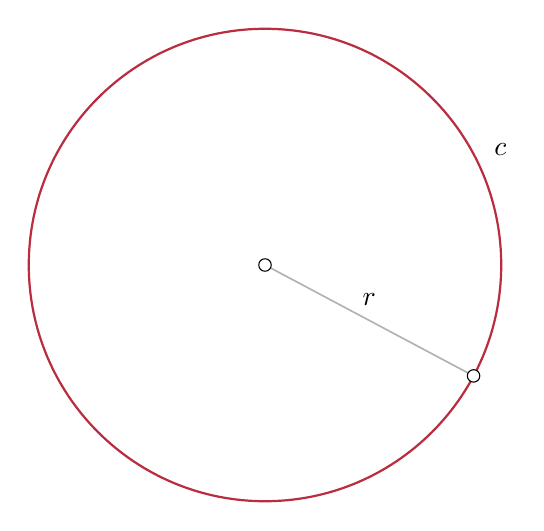
\begin{tikzpicture}[scale=1.5]
    % Parameter für den Radius und den Winkel der Radiuslinie
    \def\r{2.0}
    \def\angle{-28}
    
    % Vollständiger, hervorgehobener Kreis (Umfang c)
    \draw[crimsonred, thick] (0,0) circle (\r);
    
    % Zeichne die Radiuslinie
    \draw[gray!60, semithick] (0,0) -- (\angle:\r);
    
    % Beschriftung für den Radius 'r' (leicht über der Linie zentriert)
    \node[above, yshift=2pt] at (\angle:0.5*\r) {$r$};
    
    % Beschriftung für den Umfang 'c' (ausserhalb des Kreises bei ca. 25 Grad)
    \node[above right, xshift=2pt] at (25:\r) {$c$};
    
    % Kleine offene Kreise an den Knotenpunkten (Mittelpunkt und Randpunkt)
    \filldraw[fill=white, draw=black, thin] (0,0) circle (1.5pt);
    \filldraw[fill=white, draw=black, thin] (\angle:\r) circle (1.5pt);
    
\end{tikzpicture}
\end{document}
